\documentclass[11pt, aspectratio=43]{beamer}

% ---- Theme ----
\usetheme{Madrid}
\usecolortheme{default}

% ---- Font: Times ----
\usepackage{mathptmx}

% ---- Packages ----
\usepackage{graphicx}
\usepackage{amsmath}
\usepackage{amsfonts}
\usepackage{amssymb}
\usepackage{booktabs}
\usepackage{textcomp}

% ---- Remove navigation symbols ----
\setbeamertemplate{navigation symbols}{}

% ---- Slide numbers ----
\setbeamertemplate{footline}[frame number]

% ---- Metadata ----
\title[MS5612 Project]{Pricing Spinny's Buyback Guarantee \\ as a Real Option}
\subtitle{MS5612 -- Real Options Valuation}
\author{Group 4}
\institute{Department of Management Studies \\ IIT Madras}
\date{\today}


\begin{document}

% ============================================================
% TITLE SLIDE
% ============================================================
\begin{frame}
    \titlepage
\end{frame}


% ============================================================
% OUTLINE
% ============================================================
\begin{frame}{Outline}
    \tableofcontents
\end{frame}


% ============================================================
\section{About Spinny}
% ============================================================

\begin{frame}{About Spinny}
    \begin{itemize}
        \item Founded in 2015; operates in the \textbf{second-hand car market}
        \item Full-stack model: buys, inspects (200-point), refurbishes, and sells used cars
        \item Revenue grew from Rs.~3,262 cr (FY23) to Rs.~4,657 cr (FY25)
        \item Net losses cut nearly in half: Rs.~820 cr $\to$ Rs.~423 cr
        \item Total funding: \$700 million
    \end{itemize}

    \vspace{0.5em}
    \textbf{Key product:} Assured Buyback program -- guarantees a predetermined resale value for up to 18 months.
\end{frame}


% ============================================================
\section{Basics of Options}
% ============================================================

\begin{frame}{What is an Option?}
    A \textbf{vanilla option} gives the buyer the right, but not the obligation, to buy or sell an asset at a specific price ($K$) on or before a set date ($T$).

    \vspace{0.8em}
    \textbf{Put option payoff at expiration:}
    \[
        \text{Payoff} = \max(K - S_T, \; 0)
    \]

    \vspace{0.8em}
    \textbf{Two main types:}
    \begin{itemize}
        \item \textbf{Call}: right to \emph{buy} -- exercise when $S_T > K$
        \item \textbf{Put}: right to \emph{sell} -- exercise when $S_T < K$
    \end{itemize}
\end{frame}


\begin{frame}{Spinny's Buyback as a Real Option}
    \textbf{Real options} apply financial option theory to business decisions.

    \vspace{0.8em}
    Spinny's buyback guarantee $=$ \textbf{Put option} for the customer:

    \vspace{0.5em}
    \begin{table}
        \centering
        \begin{tabular}{@{}ll@{}}
            \toprule
            \textbf{Financial Option} & \textbf{Spinny Buyback} \\
            \midrule
            Underlying asset ($S$) & The used car \\
            Strike price ($K$) & Guaranteed buyback amount \\
            Expiration ($T$) & Return window (3 months) \\
            Put payoff & $\max(K - S_T, \; 0)$ \\
            \bottomrule
        \end{tabular}
    \end{table}

    \vspace{0.5em}
    The customer has the right, but not the obligation, to sell the car back at $K$.
\end{frame}


% ============================================================
\section{The Buyback Offer}
% ============================================================

\begin{frame}{Option Parameters}
    \begin{table}
        \centering
        \begin{tabular}{@{}ll@{}}
            \toprule
            \textbf{Parameter} & \textbf{Value} \\
            \midrule
            Model Name & Mahindra Bolero Neo Plus P10 \\
            Model Year & 2024 \\
            Selling Price ($S_0$) & Rs.~12,83,903 \\
            Buyback Price ($K$) & Rs.~11,55,641 \\
            Time to Maturity ($T$) & 3 months \\
            Risk-free Rate ($r$) & 5.26\% p.a. \\
            Depreciation ($\delta$) & 10\% p.a. \\
            Volatility ($\sigma$) & 15\% p.a.\ (base case) \\
            \bottomrule
        \end{tabular}
    \end{table}

    \vspace{0.5em}
    $K / S_0 \approx 0.90$ -- the car must lose $\sim$10\% for the put to be in the money.
\end{frame}


% ============================================================
\section{Pricing: Fundamental Approach}
% ============================================================

\begin{frame}{Pricing Using Fundamentals}
    At 10\% p.a.\ depreciation, the 3-month decline is:
    \[
        1 - (0.9)^{0.25} \approx 2.60\%
    \]

    Expected market value after 3 months:
    \[
        S_T = 12{,}83{,}903 \times 0.974 \approx \text{Rs.}~12{,}50{,}526
    \]

    \vspace{0.3em}
    Since $S_T \gg K$, the \textbf{intrinsic value is zero} under pure depreciation.

    \vspace{0.5em}
    But if we only value the option as the discounted value of depreciation. 
    
    We get, option value as $33,377 \times e^{- 0.0526 \times 0.25} = 32,941$.


\end{frame}


% ============================================================
\section{Pricing: Binomial Model}
% ============================================================

\begin{frame}{Binomial Model -- Setup}
    Divide option life $T$ into $N$ steps of $\Delta t = T/N$. At each step:
    \[
        u = e^{\sigma \sqrt{\Delta t}}, \qquad d = \frac{1}{u}
    \]

    Risk-neutral probability:
    \[
        p = \frac{e^{r \Delta t} - d}{u - d}
    \]

    Stock price at node $(i, j)$:
    \[
        S_{i,j} = S_0 \cdot u^j \cdot d^{(i-j)}
    \]

    Backward induction:
    \[
        V_{i,j} = e^{-r \Delta t} \left[ p \cdot V_{i+1,j+1} + (1-p) \cdot V_{i+1,j} \right]
    \]
\end{frame}


\begin{frame}{Standard Binomial -- Result}
    With $S_0 = \text{Rs.}~12{,}83{,}903$, $K = \text{Rs.}~11{,}55{,}641$, $\sigma = 30\%$, $N = 100$:

    \vspace{0.8em}
    \begin{table}
        \centering
        \begin{tabular}{@{}ll@{}}
            \toprule
            Up factor ($u$) & 1.015113 \\
            Down factor ($d$) & 0.985112 \\
            Risk-neutral $p$ & 0.502917 \\
            \midrule
            \textbf{Put Option Value} & \textbf{Rs.~20,513} \\
            Stock + Put Value & Rs.~13,04,416 \\
            \bottomrule
        \end{tabular}
    \end{table}
\end{frame}


\begin{frame}{Adding Deterministic Depreciation}
    A used car is not a stock -- it \textbf{deterministically depreciates}.

    \vspace{0.5em}
    Modified stock price at each node:
    \[
        S_{i,j} = S_0 \cdot \underbrace{(1 - \delta)^{t_i}}_{\text{depreciation}} \cdot \underbrace{u^j \cdot d^{(i-j)}}_{\text{stochastic}}
    \]

    \vspace{0.5em}
    Since depreciation is explicitly in the stock price, we use the \emph{standard} risk-neutral probability $p$. (no adjustment is needed)

    \vspace{0.5em}
    Over 90 days, the depreciation factor is:
    \[
        (0.9)^{0.25} \approx 0.974 \quad \text{(base value drops $\sim$2.6\%)}
    \]
\end{frame}


\begin{frame}{Binomial Heatmap -- Sensitivity Analysis}
    \begin{figure}
        \centering
        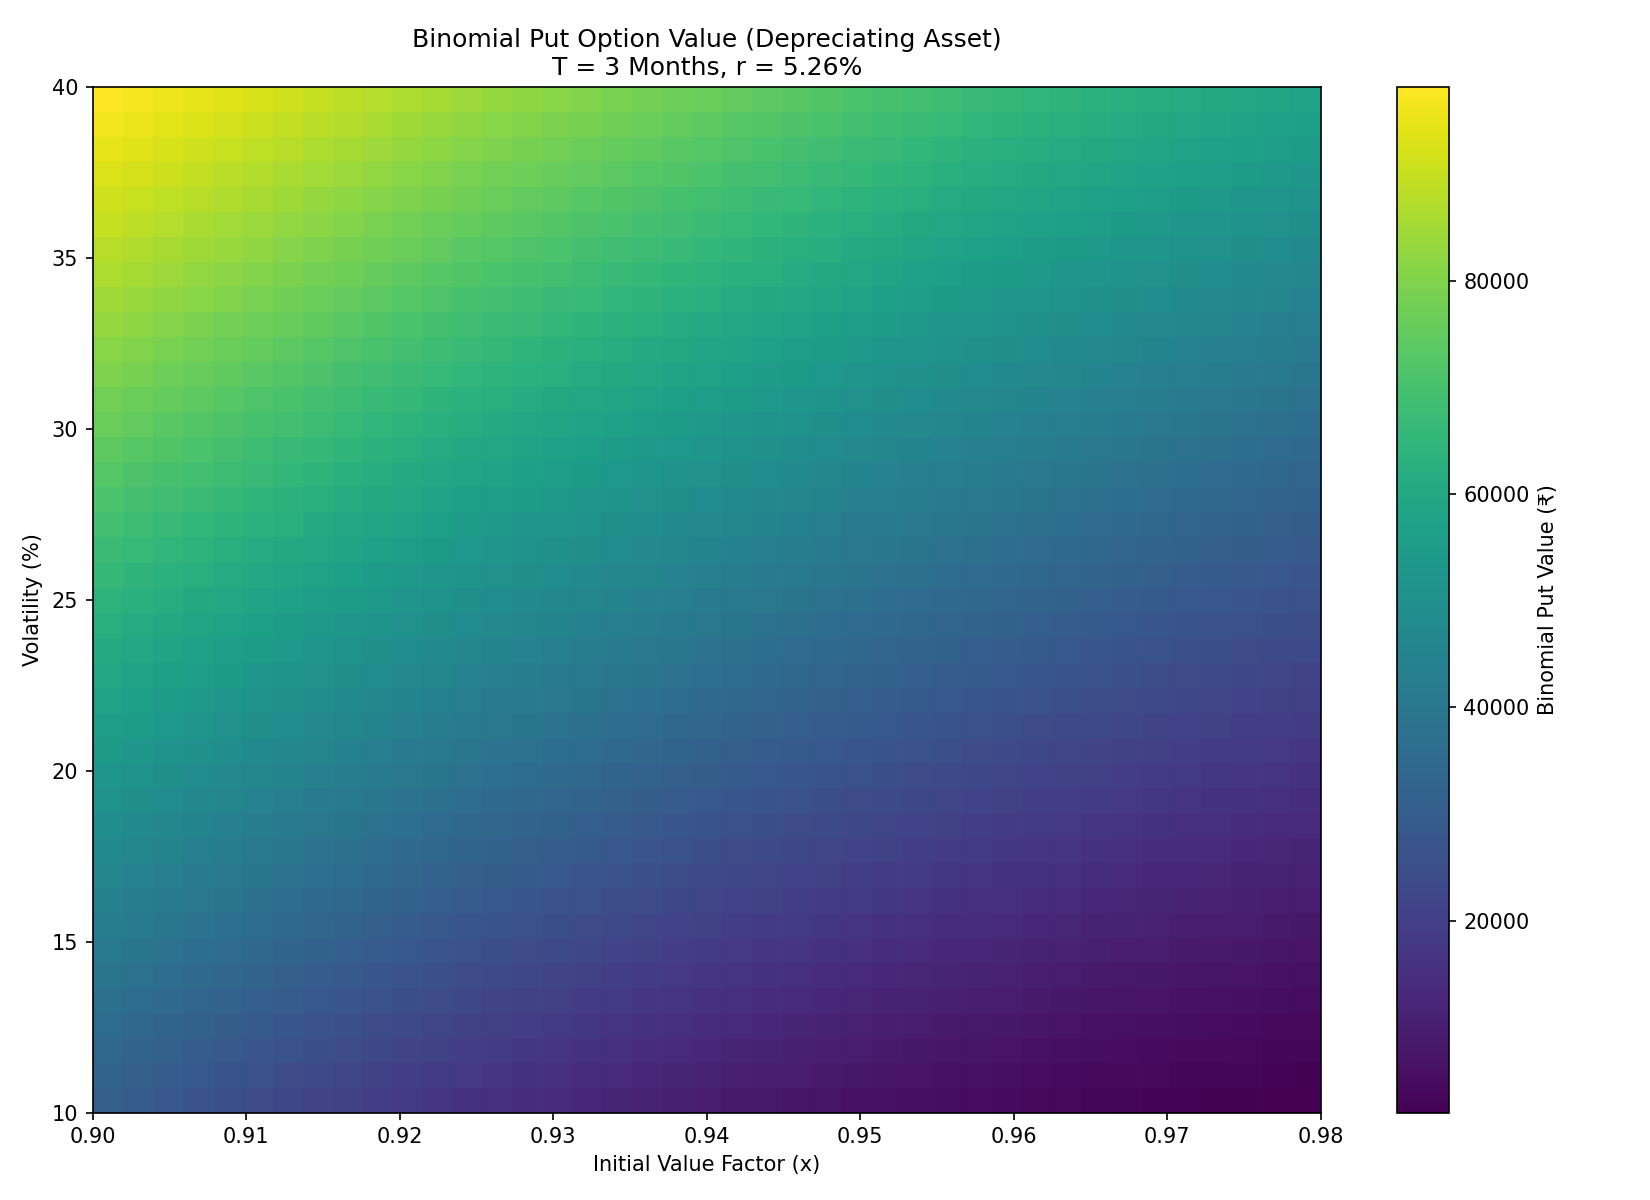
\includegraphics[width=0.72\textwidth]{fig_cell2.png}
        \caption{Put value across value factor ($x$) and volatility ($\sigma$). Range: Rs.~1,449 to Rs.~93,801.}
    \end{figure}
\end{frame}


\begin{frame}{Binomial Tree Visualisation}
    \begin{figure}
        \centering
        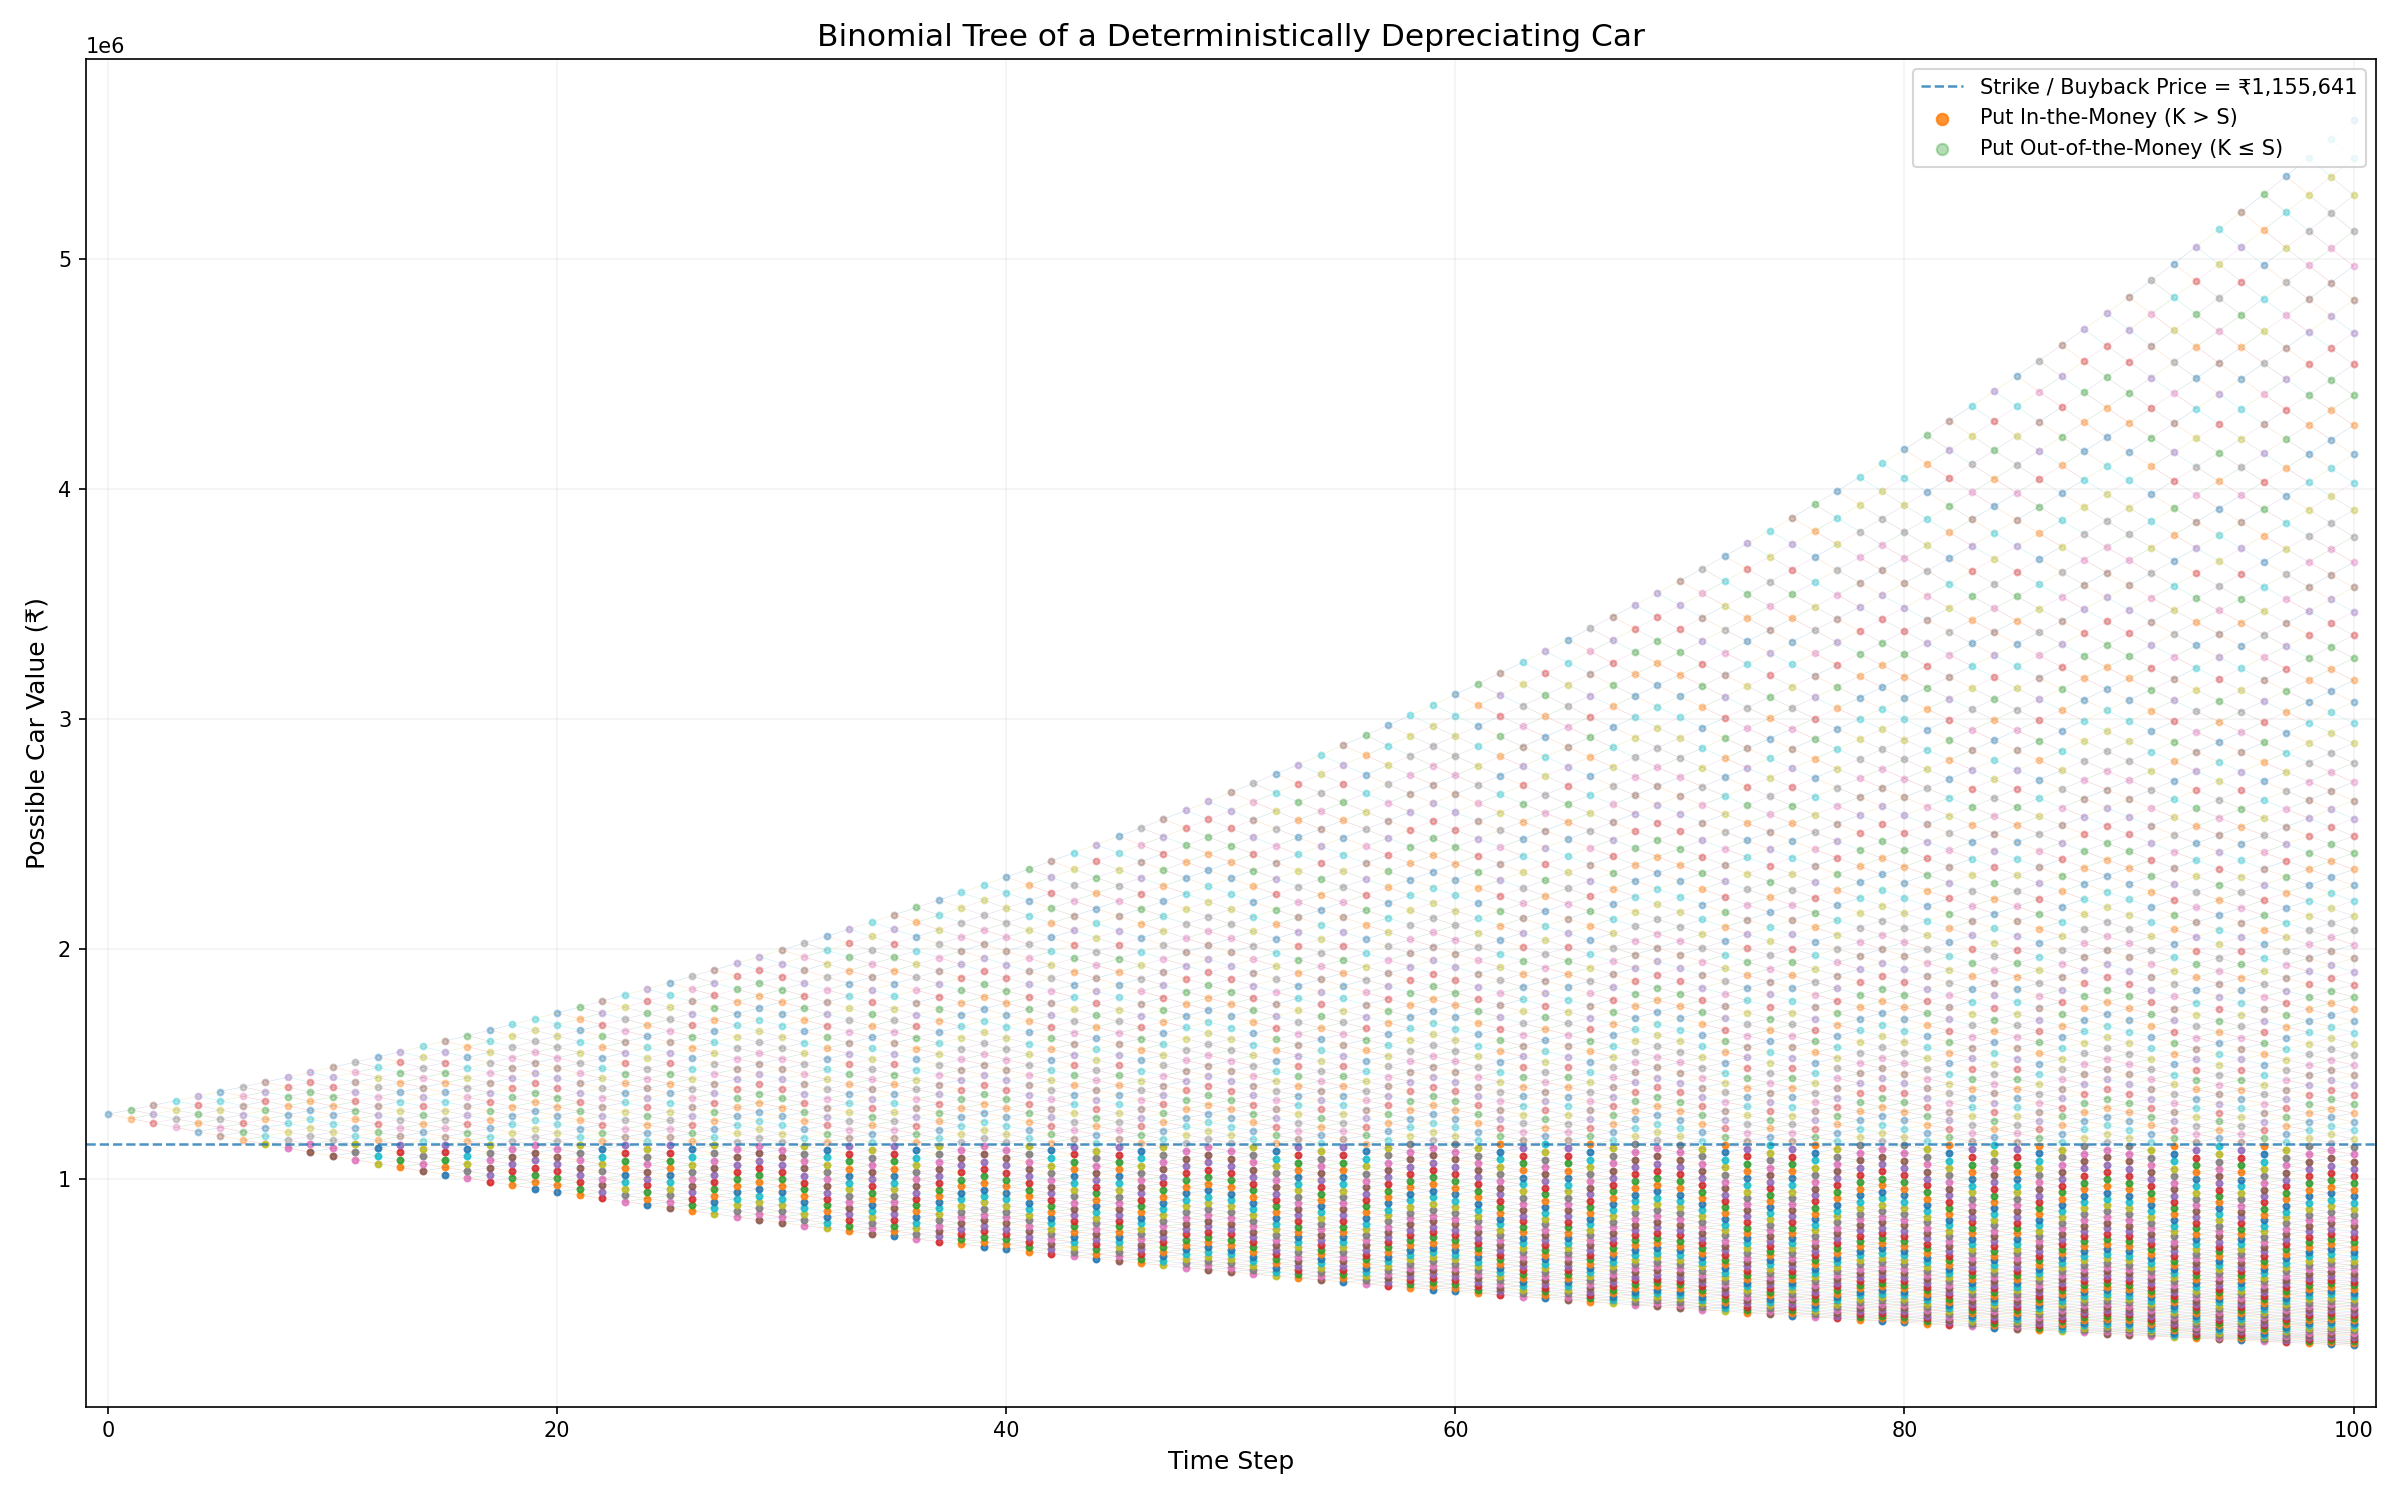
\includegraphics[width=0.82\textwidth]{fig_cell3.png}
        \caption{100-period binomial tree. Brighter nodes = put in the money ($K > S$). Dashed line = buyback price.}
    \end{figure}
\end{frame}


% ============================================================
\section{Pricing: Black-Scholes-Merton}
% ============================================================

\begin{frame}{BSM Put Formula}
    \[
        P = K \, e^{-rT} \, N(-d_2) \;-\; S_0 \, N(-d_1)
    \]
    where:
    \[
        d_1 = \frac{\ln(S_0/K) + (r + \tfrac{1}{2}\sigma^2)\,T}{\sigma\sqrt{T}}, \qquad d_2 = d_1 - \sigma\sqrt{T}
    \]

    \vspace{0.5em}
    Sample values at $\sigma = 25\%$ (no depreciation):
    \begin{itemize}
        \item $S = \text{Rs.}~12{,}83{,}903$: Put $\approx$ Rs.~12,496
        \item $S = \text{Rs.}~11{,}55{,}641$ (ATM): Put $\approx$ Rs.~46,307
    \end{itemize}
\end{frame}


\begin{frame}{BSM Heatmap -- No Depreciation}
    \begin{figure}
        \centering
        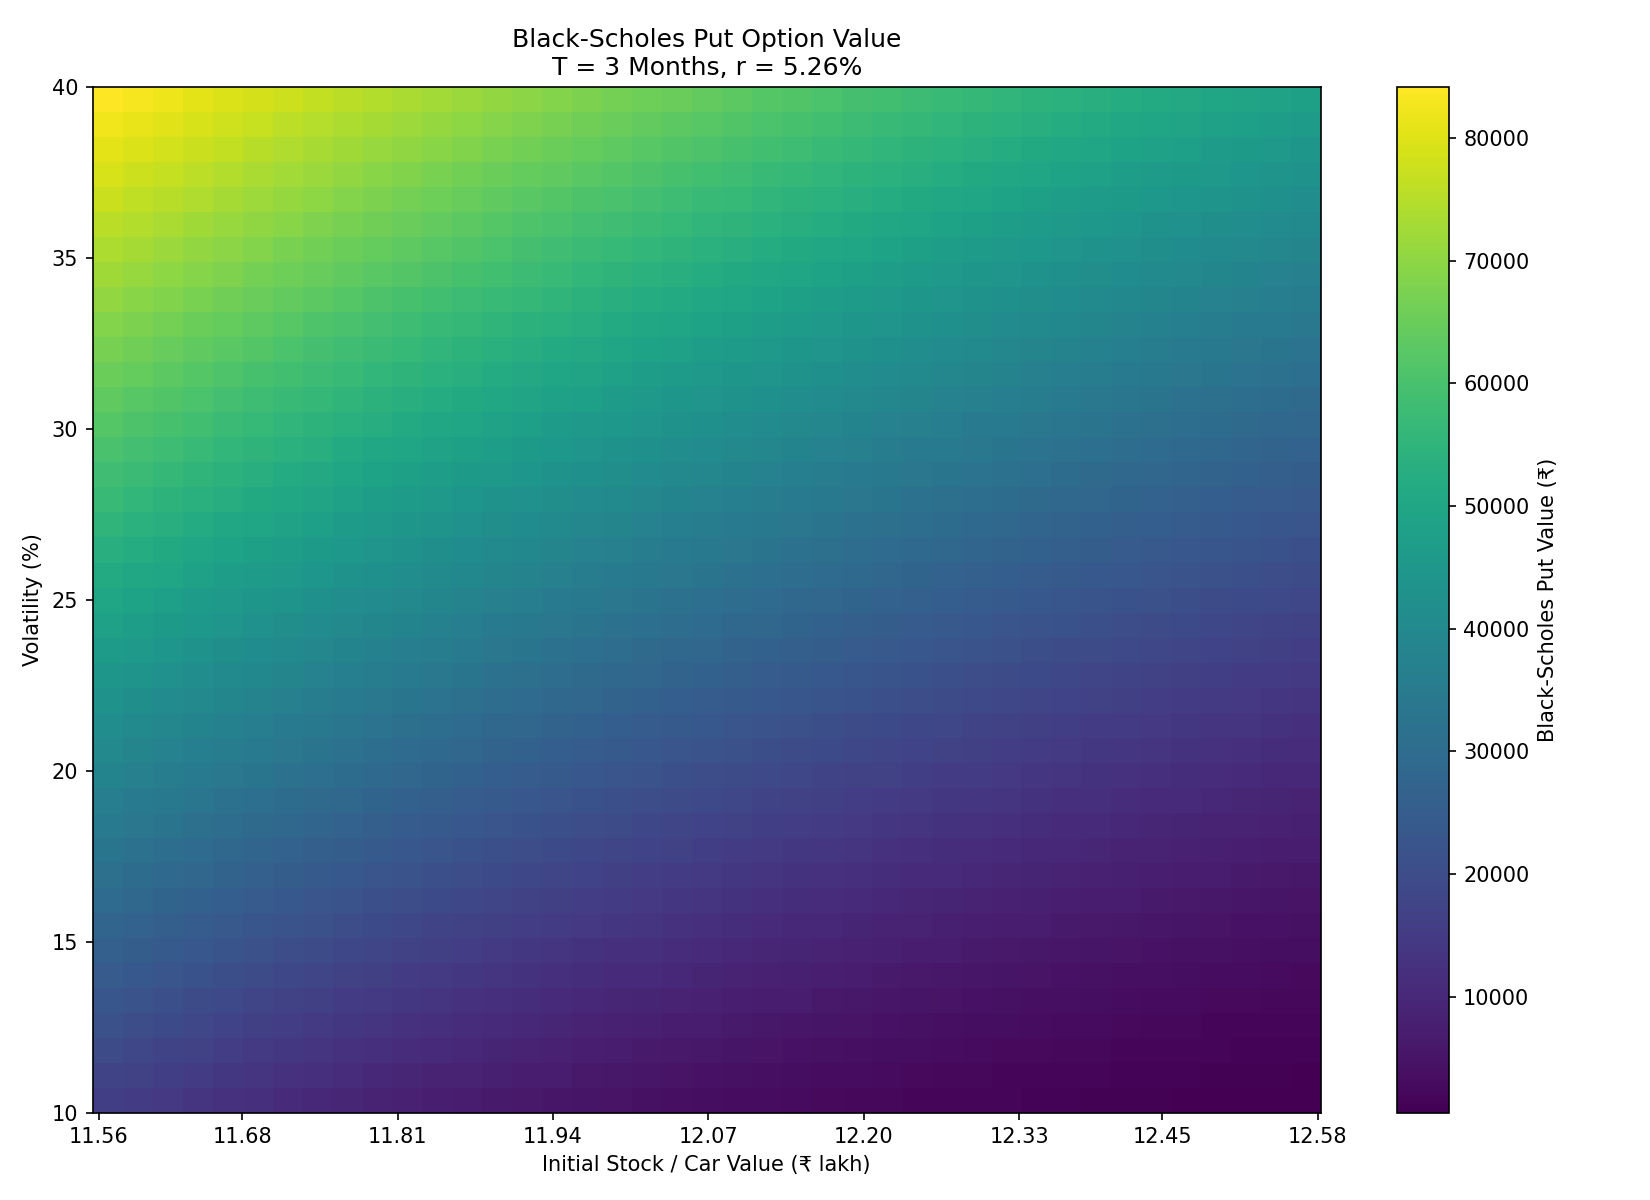
\includegraphics[width=0.72\textwidth]{fig_cell4.png}
        \caption{BSM put value without depreciation. Range: Rs.~385 to Rs.~80,208.}
    \end{figure}
\end{frame}


\begin{frame}{Incorporating Depreciation into BSM}
    Convert 10\% annual depreciation to a continuous decay rate:
    \[
        q = -\ln(1 - \delta) = -\ln(0.9) \approx 10.536\% \text{ p.a.}
    \]

    \vspace{0.5em}
    Modified BSM put formula:
    \[
        P = K \, e^{-rT} \, N(-d_2) \;-\; S_0 \, e^{-qT} \, N(-d_1)
    \]
    \[
        d_1 = \frac{\ln(S_0/K) + (r - q + \tfrac{1}{2}\sigma^2)\,T}{\sigma\sqrt{T}}
    \]

    \vspace{0.5em}
    Mathematically equivalent to a put on a \textbf{dividend-paying stock}, with $q$ as the dividend yield.
\end{frame}


\begin{frame}{BSM Heatmap -- With Depreciation}
    \begin{figure}
        \centering
        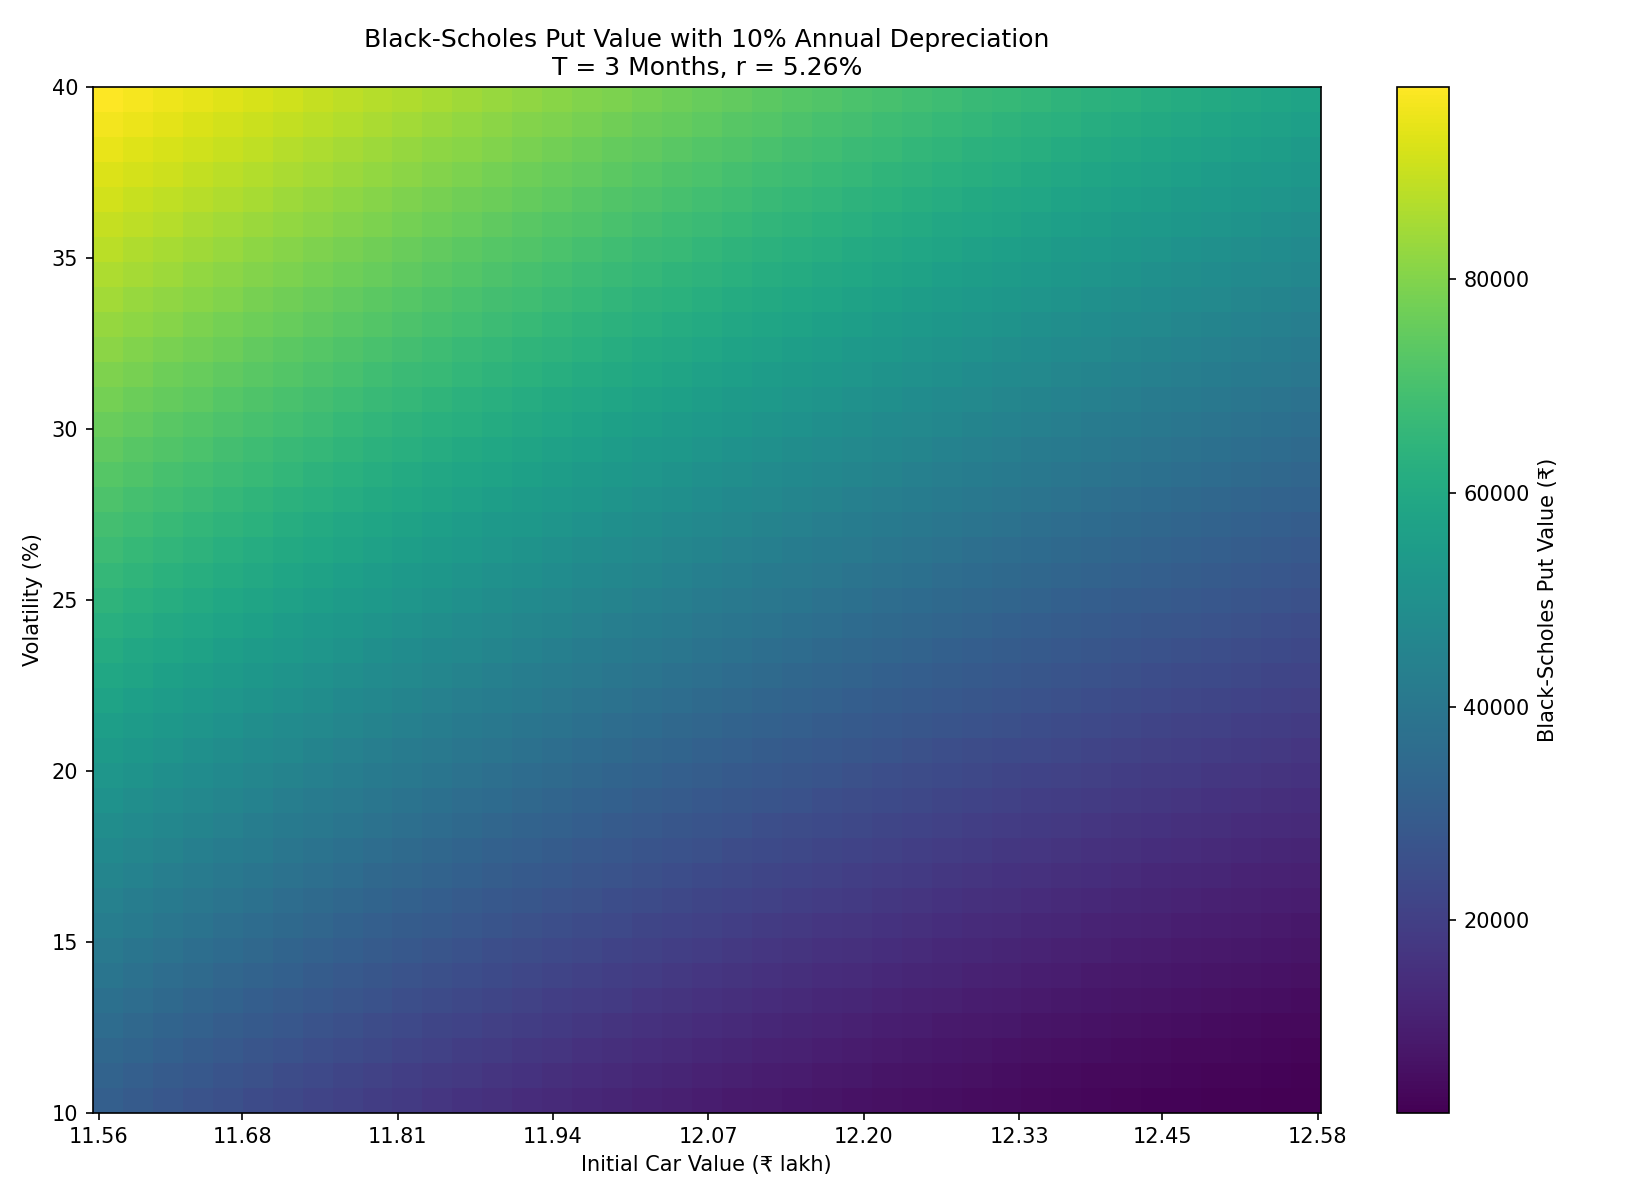
\includegraphics[width=0.72\textwidth]{fig_cell5.png}
        \caption{BSM put value with 10\% depreciation. Range: Rs.~1,455 to Rs.~93,629. Closely matches the binomial heatmap.}
    \end{figure}
\end{frame}


\begin{frame}{BSM Values at $S_0 = \text{Rs.}~12{,}83{,}903$ (With Depreciation)}
    \begin{table}
        \centering
        \begin{tabular}{@{}cc@{}}
            \toprule
            \textbf{Volatility} & \textbf{Put Value (Rs.)} \\
            \midrule
            10\% & 535 \\
            20\% & 10,116 \\
            25\% & 18,139 \\
            30\% & 27,266 \\
            40\% & 47,364 \\
            \bottomrule
        \end{tabular}
    \end{table}

    \vspace{0.5em}
    At the base-case volatility of 15\%, the option value is modest ($\sim$Rs.~535). At more realistic used-car market volatilities (25--30\%), it rises to Rs.~18,000--27,000.
\end{frame}


% ============================================================
\section{Right to Abandon}
% ============================================================

\begin{frame}{Buyback as a Right to Abandon}
    In real-options theory, the right to abandon an investment $=$ \textbf{put option} on the project value with salvage value as the strike.

    \vspace{0.8em}
    For a Spinny customer:
    \begin{itemize}
        \item Buying a used car $=$ investing in a depreciating asset
        \item Buyback guarantee $=$ guaranteed exit route
        \item If market value drops below $K$, exercise the ``abandonment option''
    \end{itemize}

    \vspace{0.8em}
    Total value of the car with the guarantee:
    \[
        \text{Total Security Value} = S_0 + P_0
    \]
    \[
        \text{Value of Embedded Put} = \text{Total Security Value} - S_0
    \]

    Base case (standard binomial): Rs.~13,04,416 total $\Rightarrow$ guarantee adds Rs.~20,513.
\end{frame}


% ============================================================
\section{Consolidation}
% ============================================================

\begin{frame}{Consolidated Pricing}
    \begin{table}
        \centering
        \small
        \begin{tabular}{@{}lcc@{}}
            \toprule
            \textbf{Method} & \textbf{Volatility} & \textbf{Put Value (Rs.)} \\
            \midrule
            Fundamental (10\% dep.) & -- & 32,941 \\
            Standard Binomial & 30\% & 20,513 \\
            BSM (no depreciation) & 25\% & 12,496 \\
            BSM (with depreciation) & 25\% & 18,139 \\
            BSM (with depreciation) & 30\% & 27,266 \\
            BSM (with depreciation) & 15\% & 535 \\
            \bottomrule
        \end{tabular}
    \end{table}

    \vspace{0.5em}
    Incorporating depreciation \textbf{significantly increases} the put value. At realistic volatilities (15--30\%), the guarantee is worth Rs.~500 to Rs.~27,000.
\end{frame}


\begin{frame}{How Would Spinny Price This?}
    Spinny's internal pricing would additionally factor in:

    \vspace{0.5em}
    \begin{itemize}
        \item Expected depreciation and buy-sell spread
        \item Inspection and reconditioning costs upon return
        \item Probability that a customer actually exercises (exercise rate)
        \item Cost of capital for the repurchase commitment
        \item Psychological value to the customer (marketing tool)
    \end{itemize}

    \vspace{0.8em}
    The 10\% haircut ($K \approx 0.90 \times S_0$) covers expected depreciation $+$ margin for operational costs and adverse selection.
\end{frame}


% ============================================================
\section{Conclusion}
% ============================================================

\begin{frame}{Conclusion}
    \begin{itemize}
        \item Spinny's buyback guarantee $\equiv$ \textbf{European put option} on a deterministically depreciating asset

        \vspace{0.5em}
        \item Three pricing methods yield consistent results: fundamental, binomial (with depreciation), and BSM (with depreciation)

        \vspace{0.5em}
        \item Key insight: deterministic depreciation \textbf{increases} the put value -- a depreciating asset is more likely to fall below the guaranteed floor

        \vspace{0.5em}
        \item Option value ranges from $\sim$Rs.~500 (low $\sigma$) to $\sim$Rs.~93,000 (high $\sigma$, low $x$)

        \vspace{0.5em}
        \item Dual purpose for Spinny: marketing tool (reduces buyer anxiety) $+$ financial obligation (must be carefully priced)
    \end{itemize}
\end{frame}


\begin{frame}{}
    \centering
    \vspace{2em}
    {\Huge Thank You}

    \vspace{1.5em}
    {\large Questions?}

    \vspace{2em}
    {\small Ajith, Hardik, Lokesh, \& Vikranth}
\end{frame}


\end{document}